\subsection{DCM}

\subsubsection{Model selection}
In order to choose  parsimonious models with good performance, two different types of models are considered, namely, Full models, which contain all the available covariates (weather, distances, lockdown, holiday), and Selected models, which include only those covariates that are significant. The model selection was carried out on the univariate spatio-temporal process related to pickups, on the univariate spatio-process process related to trip duration and on the bivariate spatio-temporal process (pickup, trip duration). After obtaining the various models, we want to evaluate their performance in comparison to the full models and their predictive ability through the Cross Validation (table \ref{Cross-validation mean squared errors DCM}).

\begin{table}
	\centering
	\renewcommand\arraystretch{1.3}
	\begin{tabular}{c|cc|cc}
		\hline
		\multicolumn{1}{l|}{} & \multicolumn{2}{c|}{\textit{CV MSE, full model}} & \multicolumn{2}{c}{\textit{CV MSE, selected model} }\\ 
		\hline
		\textit{Model} & \multicolumn{1}{c|}{\textit{Pickups}} & \textit{Trip duration} & \multicolumn{1}{c|}{\textit{Pickups}} & \textit{Trip duration} \\ 
		\hline
		\textbf{2-variate } & \multicolumn{1}{c|}{0.9870}  & 0.9624   & \multicolumn{1}{c|}{0.6584}  & 0.8221   \\ 
		\hline
		\textbf{1-variate } & \multicolumn{1}{c|}{0.4654}  & 0.7825   & \multicolumn{1}{c|}{0.6685}  & 0.7868   \\ 
		\hline
	\end{tabular}
	\caption[MSE concerning cross-validation in log-standardized scale for response variables (DCM)]{MSE concerning cross-validation in log-standardized scale for response variables, DCM.}
	\label{Cross-validation mean squared errors DCM}
\end{table}

\noindent
In table \ref{Log-likelihoods DCM} we compares the models' likelihood and we can see the pickups selective univariate model have the lowest log-likelihoods while the bivariate selected model have the highest.

\begin{table}
	\centering
	\renewcommand\arraystretch{1.3}
	\begin{tabular}{c|c|c}
		\hline
		\textit{Model} &\textit{Full} & \textit{Selected} \\ 
		\hline
		\textbf{2-variate } & -6106.405  & -7491.195    \\ 
		\hline
		\textbf{1-variate pickups } & -3512.167  & -3122.354    \\ 
		\hline
		\textbf{1-variate trip duration} & -4536.846  & -4309.739   \\ 
		\hline
	\end{tabular}
	\caption[Log-likelihoods of the six models (DCM)]{Log-likelihoods of the six models, DCM.}
	\label{Log-likelihoods DCM}
\end{table}

\subsubsection{Model analysis}

Figure \ref{Trend_zeta_latente univariato} shows the trend of the latent z interacting with the covariates:
\begin{itemize}
	\item $z_{1}$, which indicates the trend of the pickups is a significant variable that has a positive effect both on the number of rentals and on the average daily rental duration.
	\item $z_{2}$, which indicates the distance. The trend is always positive therefore it brings a decrease in the number of pickups
	\item $z_{3}$ , which indicates the holidays and not affect the increase of pickups.
\end{itemize}

\begin{figure}
	\centering
	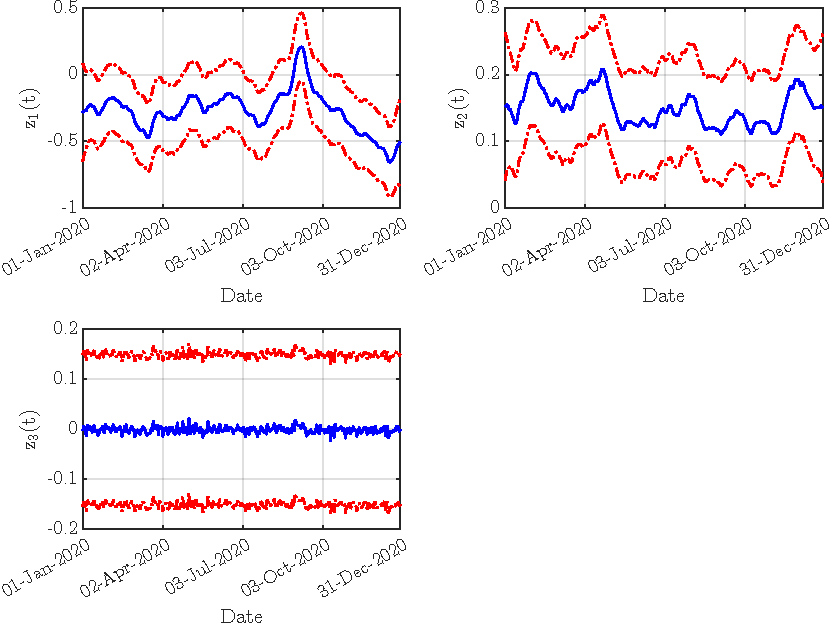
\includegraphics[height=222px]{Images/Data analysis/DCM/Trend_z_pickups.pdf}
	\caption[Estimated $z_{1}(t)$,  $z_{2}(t)$ and $z_{3}(t)$ by Kalman smoother in the univariate model for pickups (DCM)]{estimated $z_{1}(t)$,  $z_{2}(t)$ and $z_{3}(t)$ by Kalman smoother in the univariate model for pickups.}
	\label{Trend_zeta_latente univariato}
	
\end{figure}

\noindent
Figure \ref{Trend_zeta_latente} shows the trend of the latent z interacting with the covariates:
\begin{itemize}
	\item $z_{1}$, which indicates the trend of the pickups.
	\item $z_{2}$, is refers to the distance. in comparison to the univariate case it can be noted  an decrease in pickups.
	\item $z_{3}$ , which indicates the trend of the average of trip duration
	\item $z_{4}$ , which indicates the distance and not affect the increase of the average trip duration.
\end{itemize}

\begin{figure}
	\centering
	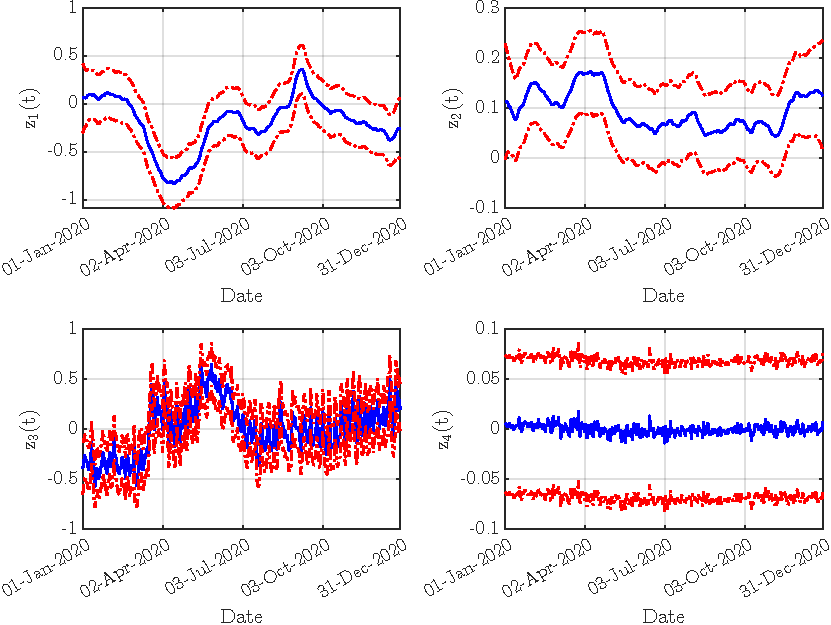
\includegraphics[height=222px]{Images/Data analysis/DCM/Trend_z_biv.pdf}
	\caption[Estimated $z_{1}(t)$,  $z_{2}(t)$ and $z_{3}(t)$ by Kalman smoother in the bivariate model (DCM)]{estimated $z_{1}(t)$,  $z_{2}(t)$ and $z_{3}(t)$ by kalman smoother in the bivariate model.}
	\label{Trend_zeta_latente}
\end{figure}

\noindent
The most significant coefficients $\boldsymbol{\hat{\beta}}$ are shown in the  table \ref{z_latent trend}, it can be seen that both models the most significant coefficients are $\boldsymbol{\hat{\beta}_{temp}}$ and $\boldsymbol{\hat{\beta}_{UV}}$
 \begin{table}
	\centering
	\renewcommand\arraystretch{1.3}
	\begin{tabular}{c|c|c|c|c|c|c|c}
		\hline
		\textit{} & $\boldsymbol{\hat{\beta}_{const}}$ & $\boldsymbol{\hat{\beta}_{temp}}$ & $\boldsymbol{\hat{\beta}_{rain}}$ & $\boldsymbol{\hat{\beta}_{dist}}$ & $\boldsymbol{\hat{\beta}_{Holiday}}$ & $\boldsymbol{\hat{\beta}_{Lock}}$ & $\boldsymbol{\hat{\beta}_{UV}}$   \\
		\hline
		\textbf{2-variate pickups} & \num{-0.109} & \num{+0.264} & \num{-0.054} & \num{+0.089} & \num{+0.222} &  & \num{+0.154}  \\
		\hline
		\textbf{2-variate trip duration} & \num{-0.071} & \num{+0.310} &  & \num{-0.064} & \num{-0.048} & \num{-0.171} & \num{+0.145}  \\
		\hline
		\textbf{1-variate pickups} & \num{+0.079} & \num{+0.269} & \num{-0.053} & \num{-0.206} & \num{+0.001} & \num{-0.693} & \num{+0.104}\\
		\hline
	\end{tabular}
	\caption[Estimated $\boldsymbol{\beta}$ for the bivariate model and 1-variate pickups (DCM)]{estimated $\boldsymbol{\beta}$ for the bivariate model and \num{1}-variate pickups.}
	\label{z_latent trend}
\end{table}